%% Run LaTeX on this file several times to get Table of Contents,
%% cross-references, and citations.

\documentclass[11pt]{book}
\usepackage{gvv}
\usepackage{gvv-book-bkup}
%\usepackage{Wiley-AuthoringTemplate}
\usepackage[sectionbib,authoryear]{natbib}% for name-date citation comment the below line
%\usepackage[sectionbib,numbers]{natbib}% for numbered citation comment the above line

%%********************************************************************%%
%%       How many levels of section head would you like numbered?     %%
%% 0= no section numbers, 1= section, 2= subsection, 3= subsubsection %%
\setcounter{secnumdepth}{3}
%%********************************************************************%%
%%**********************************************************************%%
%%     How many levels of section head would you like to appear in the  %%
%%				Table of Contents?			%%
%% 0= chapter, 1= section, 2= subsection, 3= subsubsection titles.	%%
\setcounter{tocdepth}{2}
%%**********************************************************************%%
\setcounter{tocdepth}{3}
%\includeonly{ch01}
\makeindex

\begin{document}

\frontmatter
%%%%%%%%%%%%%%%%%%%%%%%%%%%%%%%%%%%%%%%%%%%%%%%%%%%%%%%%%%%%%%%%
%% Title Pages
%% Wiley will provide title and copyright page, but you can make
%% your own titlepages if you'd like anyway
%% Setting up title pages, type in the appropriate names here:

\booktitle{ICSE Math}

\subtitle{Made Simple}

\AuAff{G. V. V. Sharma}

%% \\ will start a new line.
%% You may add \affil{} for affiliation, ie,
%\authors{Robert M. Groves\\
%\affil{Universitat de les Illes Balears}
%Floyd J. Fowler, Jr.\\
%\affil{University of New Mexico}
%}

%% Print Half Title and Title Page:
%\halftitlepage
\titlepage

%%%%%%%%%%%%%%%%%%%%%%%%%%%%%%%%%%%%%%%%%%%%%%%%%%%%%%%%%%%%%%%%
%%Copyright Page

\begin{copyrightpage}{2023}
%Title, etc
\end{copyrightpage}

% Note, you must use \ to start indented lines, ie,
% 
% \begin{copyrightpage}{2004}
% Survey Methodology / Robert M. Groves . . . [et al.].
% \       p. cm.---(Wiley series in survey methodology)
% \    ``Wiley-Interscience."
% \    Includes bibliographical references and index.
% \    ISBN 0-471-48348-6 (pbk.)
% \    1. Surveys---Methodology.  2. Social 
% \  sciences---Research---Statistical methods.  I. Groves, Robert M.  II. %
% Series.\\

% HA31.2.S873 2004
% 001.4'33---dc22                                             2004044064
% \end{copyrightpage}

%%%%%%%%%%%%%%%%%%%%%%%%%%%%%%%%%%%%%%%%%%%%%%%%%%%%%%%%%%%%%%%%
%% Only Dedication (optional) 

%\dedication{To my parents}

\tableofcontents

%\listoffigures %optional
%\listoftables  %optional

%% or Contributor Page for edited books
%% before \tableofcontents

%%%%%%%%%%%%%%%%%%%%%%%%%%%%%%%%%%%%%%%%%%%%%%%%%%%%%%%%%%%%%%%%
%  Contributors Page for Edited Book
%%%%%%%%%%%%%%%%%%%%%%%%%%%%%%%%%%%%%%%%%%%%%%%%%%%%%%%%%%%%%%%%

% If your book has chapters written by different authors,
% you'll need a Contributors page.

% Use \begin{contributors}...\end{contributors} and
% then enter each author with the \name{} command, followed
% by the affiliation information.

% \begin{contributors}
% \name{Masayki Abe,} Fujitsu Laboratories Ltd., Fujitsu Limited, Atsugi, Japan
%
% \name{L. A. Akers,} Center for Solid State Electronics Research, Arizona State University, Tempe, Arizona
%
% \name{G. H. Bernstein,} Department of Electrical and Computer Engineering, University of Notre Dame, Notre Dame, South Bend, Indiana; formerly of
% Center for Solid State Electronics Research, Arizona
% State University, Tempe, Arizona 
% \end{contributors}

%%%%%%%%%%%%%%%%%%%%%%%%%%%%%%%%%%%%%%%%%%%%%%%%%%%%%%%%%%%%%%%%
% Optional Foreword:

%\begin{foreword}
%\lipsum[1-2]
%\end{foreword}

%%%%%%%%%%%%%%%%%%%%%%%%%%%%%%%%%%%%%%%%%%%%%%%%%%%%%%%%%%%%%%%%
% Optional Preface:

%\begin{preface}
%\lipsum[1-1]
%\prefaceauthor{}
%\where{place\\
% date}
%\end{preface}

% ie,
% \begin{preface}
% This is an example preface.
% \prefaceauthor{R. K. Watts}
% \where{Durham, North Carolina\\
% September, 2004}

%%%%%%%%%%%%%%%%%%%%%%%%%%%%%%%%%%%%%%%%%%%%%%%%%%%%%%%%%%%%%%%%
% Optional Acknowledgments:

%\acknowledgments
%\lipsum[1-2]
%\authorinitials{I. R. S.}  

%%%%%%%%%%%%%%%%%%%%%%%%%%%%%%%%
%% Glossary Type of Environment:

% \begin{glossary}
% \term{<term>}{<description>}
% \end{glossary}

%%%%%%%%%%%%%%%%%%%%%%%%%%%%%%%%
%\begin{acronyms}
%\acro{ASTA}{Arrivals See Time Averages}
%\acro{BHCA}{Busy Hour Call Attempts}
%\acro{BR}{Bandwidth Reservation}
%\acro{b.u.}{bandwidth unit(s)}
%\acro{CAC}{Call / Connection Admission Control}
%\acro{CBP}{Call Blocking Probability(-ies)}
%\acro{CCS}{Centum Call Seconds}
%\acro{CDTM}{Connection Dependent Threshold Model}
%\acro{CS}{Complete Sharing}
%\acro{DiffServ}{Differentiated Services}
%\acro{EMLM}{Erlang Multirate Loss Model}
%\acro{erl}{The Erlang unit of traffic-load}
%\acro{FIFO}{First in - First out}
%\acro{GB}{Global balance}
%\acro{GoS}{Grade of Service}
%\acro{ICT}{Information and Communication Technology}
%\acro{IntServ}{Integrated Services}
%\acro{IP}{Internet Protocol}
%\acro{ITU-T}{International Telecommunication Unit -- Standardization sector}
%\acro{LB}{Local balance}
%\acro{LHS}{Left hand side}
%\acro{LIFO}{Last in - First out}
%\acro{MMPP}{Markov Modulated Poisson Process}
%\acro{MPLS}{Multiple Protocol Labeling Switching}
%\acro{MRM}{Multi-Retry Model}
%\acro{MTM}{Multi-Threshold Model}
%\acro{PASTA}{Poisson Arrivals See Time Averages}
%\acro{PDF}{Probability Distribution Function}
%\acro{pdf}{probability density function}
%\acro{PFS}{Product Form Solution}
%\acro{QoS}{Quality of Service}
%\acro{r.v.}{random variable(s)}
%\acro{RED}{random early detection}
%\acro{RHS}{Right hand side}
%\acro{RLA}{Reduced Load Approximation}
%\acro{SIRO}{service in random order}
%\acro{SRM}{Single-Retry Model}
%\acro{STM}{Single-Threshold Model}
%\acro{TCP}{Transport Control Protocol}
%\acro{TH}{Threshold(s)}
%\acro{UDP}{User Datagram Protocol}
%\end{acronyms}

\setcounter{page}{1}

\begin{introduction}
This book links high school coordinate geometry to linear algebra and matrix analysis through solved problems.

\end{introduction}

\mainmatter
%\chapter{Vectors}
%\section{2020}
%\subsection{10}
%\input{2020/vetors1.0.tex}
%\subsection{12}
%\input{2020/vetors2.0.tex}



\chapter{Linear Forms}
%\section{2023}
%\subsection{10}
%\input{2023/linear-10th.tex}
%\subsection{12}                                                                                                  
%\input{2023/linear-12th.tex}
%\section{2022}

\chapter{Circles}
\section{2022}
\subsection{10}
\begin{enumerate}
	\item $ABCD$ is a cyclic quadrilateral. If $\angle BAD = (2x + 5)^{\circ}$ and $\angle BCD = (x + 10)^{\circ}$ then $x$ is equal to:
		\begin{figure}[h]
			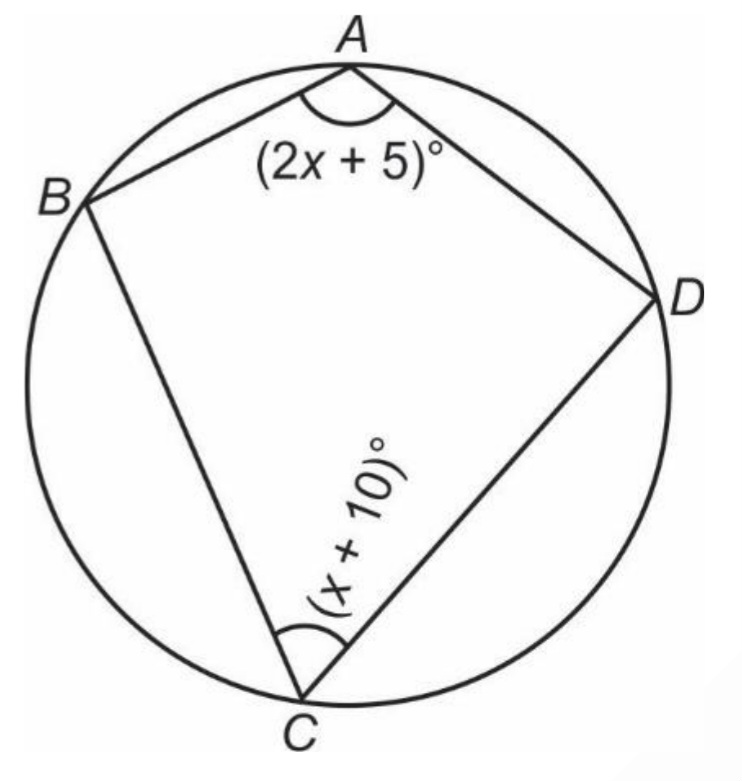
\includegraphics[width=\columnwidth]{figs/img2.jpg}
			\caption{}
			\label{figure}
		\end{figure}
		\begin{enumerate}
			\item $65^{\circ}$
			\item $45^{\circ}$
			\item $55^{\circ}$
			\item $5^{\circ}$
		\end{enumerate}
		\newpage
	\item In the given figure $O$ is the centre of the circle. $PQ$ and $PR$ are tangents and $\angle QPR = 70^{\circ}$. Calculate:
		{\begin{figure}[h]
			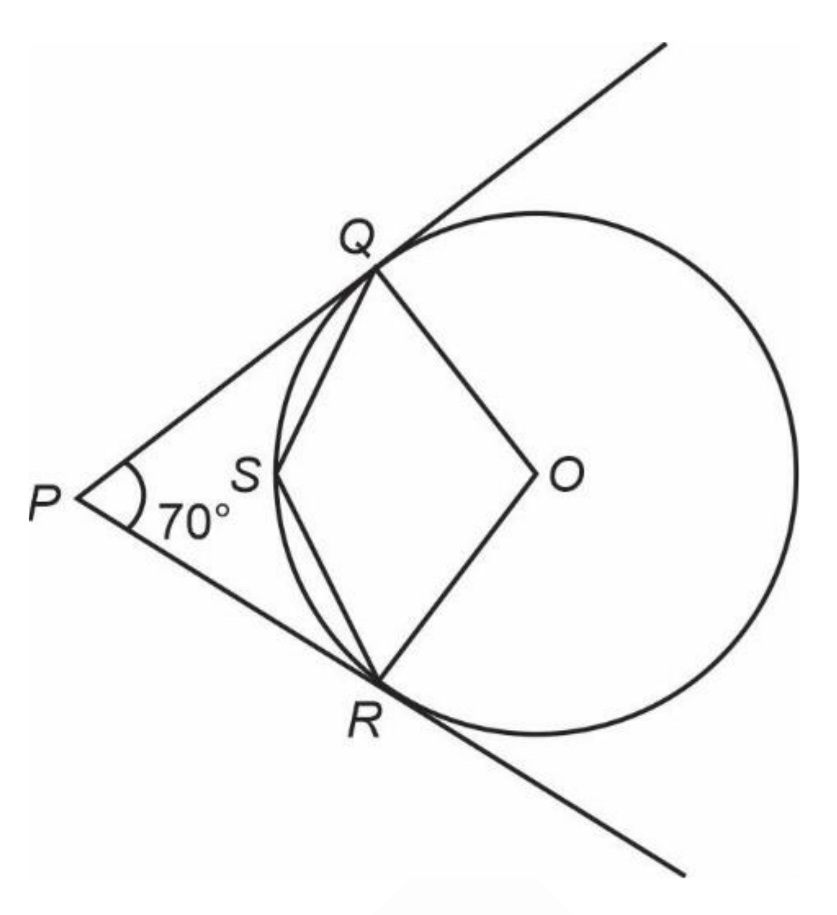
\includegraphics[width=\columnwidth]{figs/img3.jpg}
			\caption{}
			\label{figure}
		\end{figure}}
		\begin{enumerate}
			\item $\angle QOR$
			\item $\angle QSR$
		\end{enumerate}	
	\item Two chords $AB$ and $CD$ of a circle intersect extenally at $E$. if $EC = 2 cm$, $EA = 3 cm$ and $AB = 5 cm$, find the length of $CD$.
		\begin{figure}[h]
			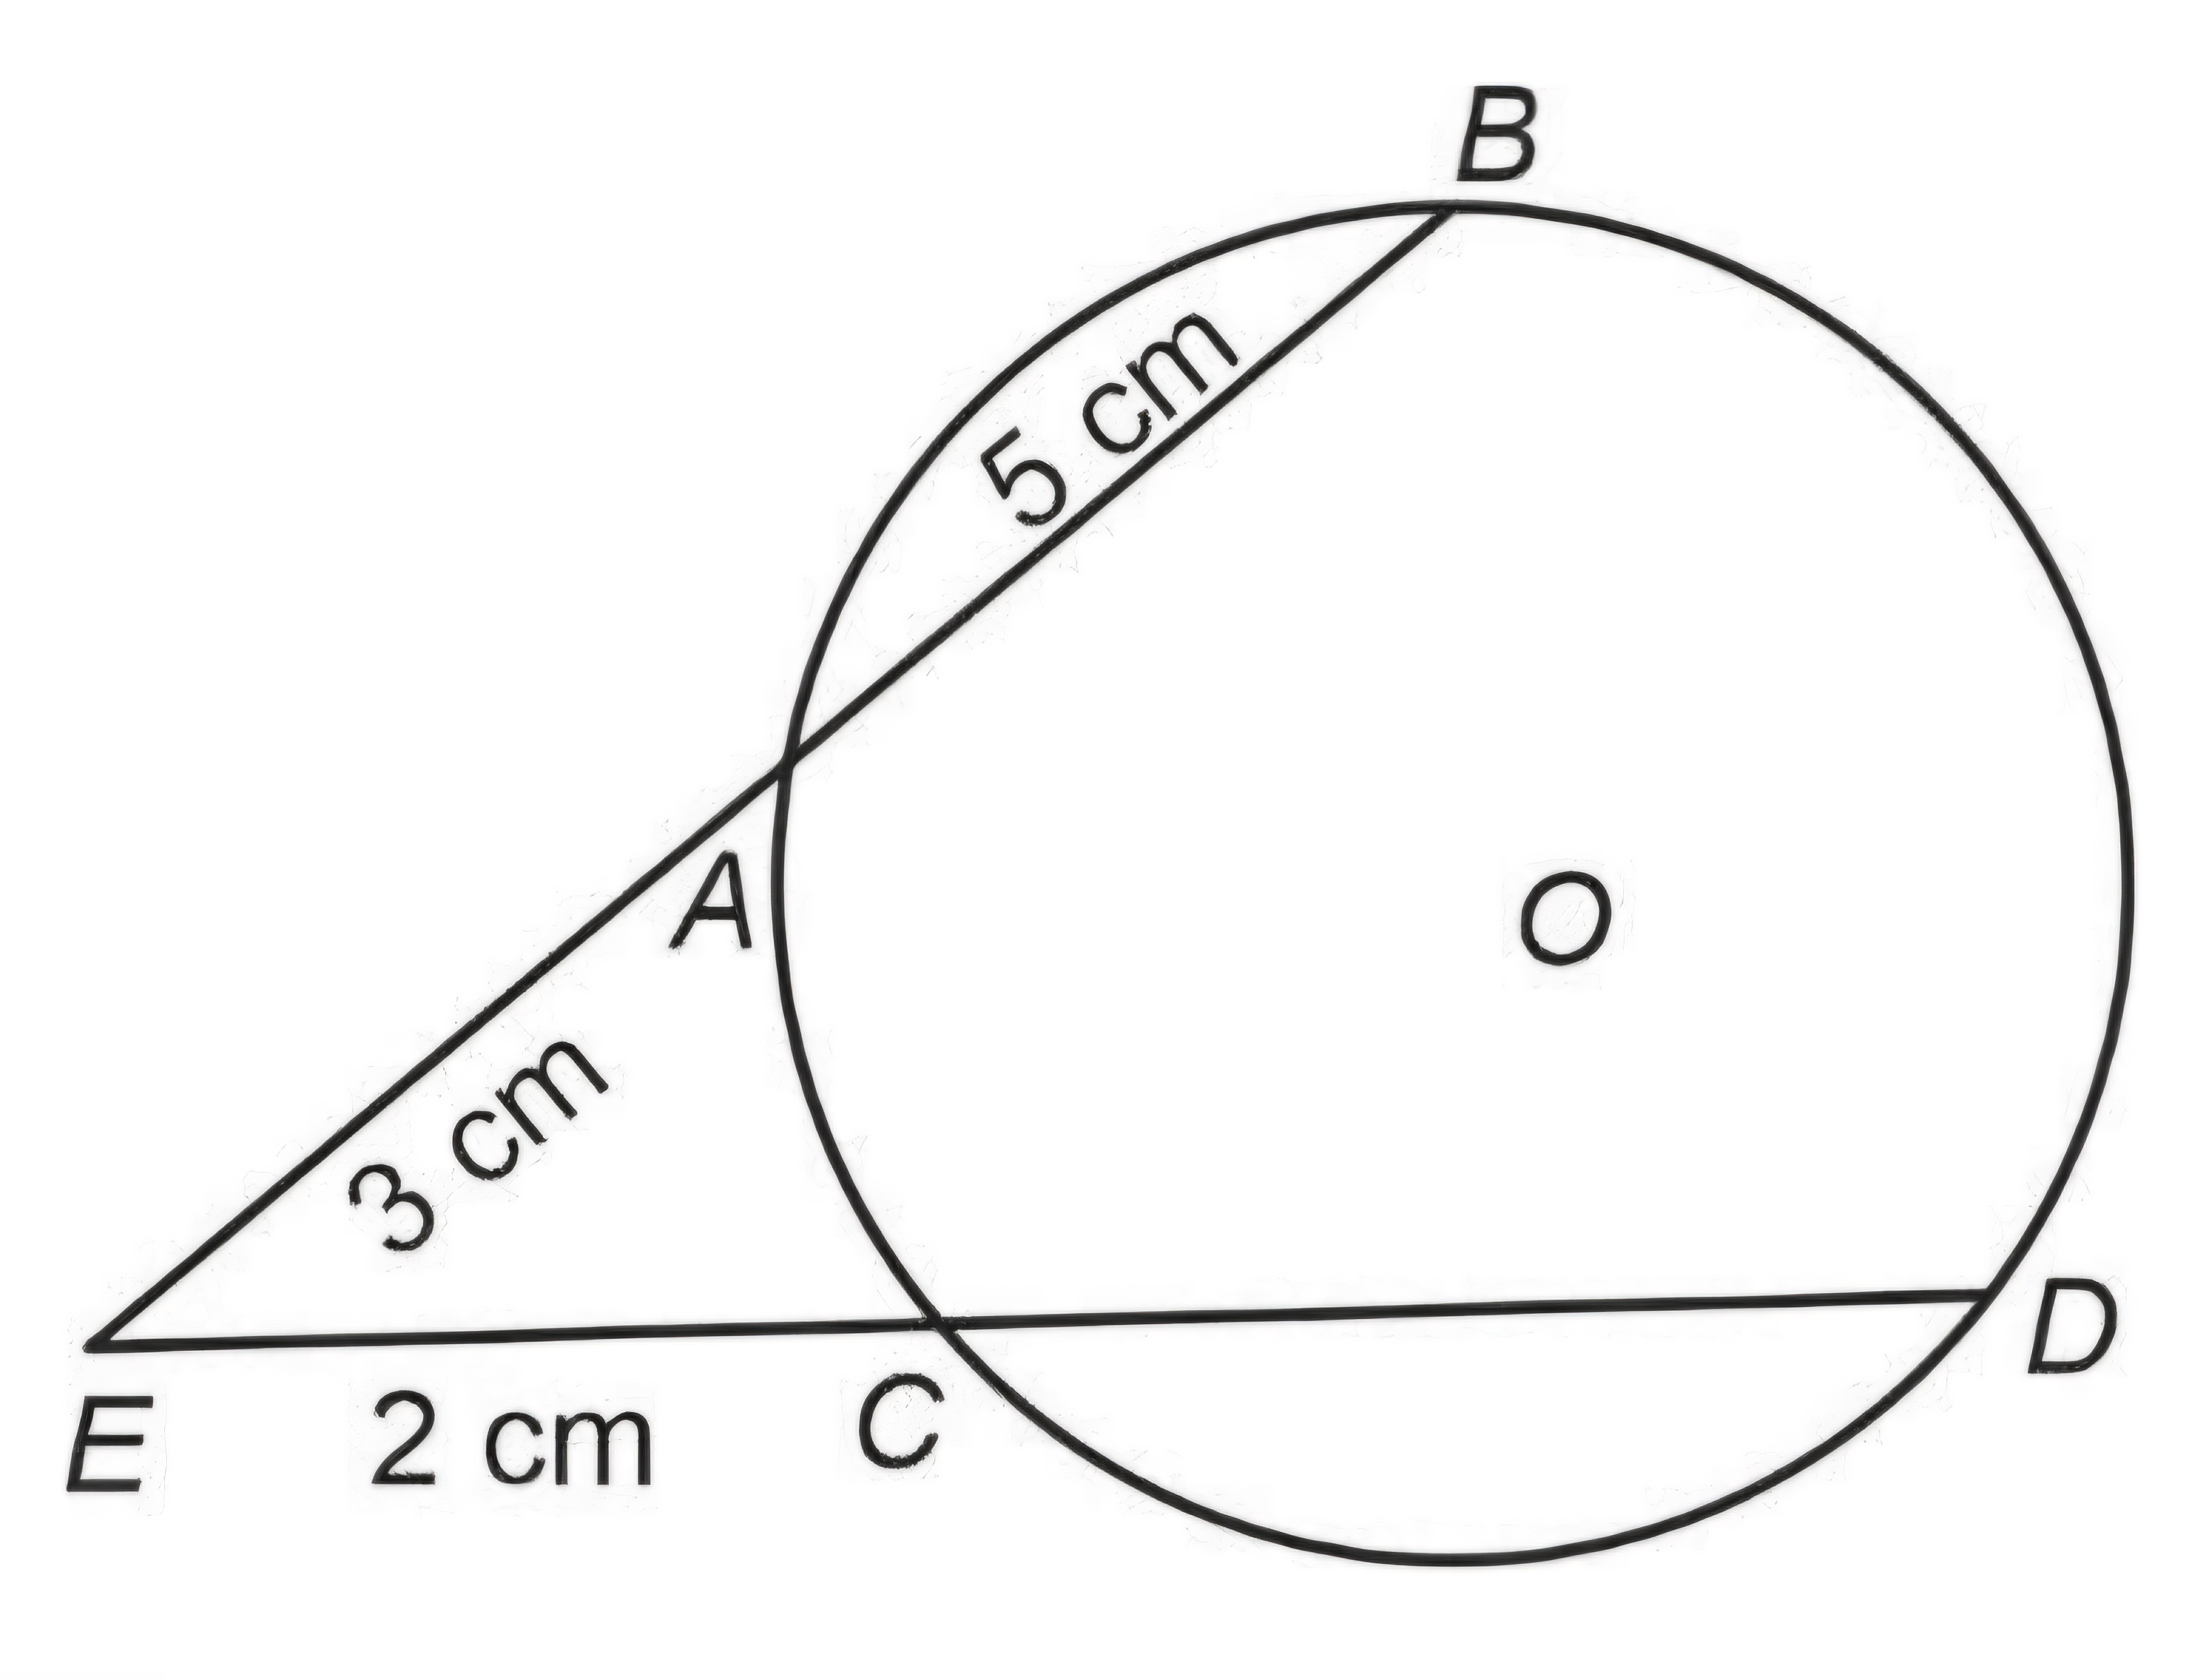
\includegraphics[width=\columnwidth]{figs/img4.jpg}
			\caption{}
			\label{figure}
		\end{figure}
		\newpage
	\item In the given figure $A,B,C$ and $D$ are points on the circle with centre $O$. Given $\angle ABS = 62^{\circ}$. Find:
		\begin{enumerate}
			\item $\angle ADC$
			\item $\angle CAB$
		\end{enumerate}
		\begin{figure}[h]
			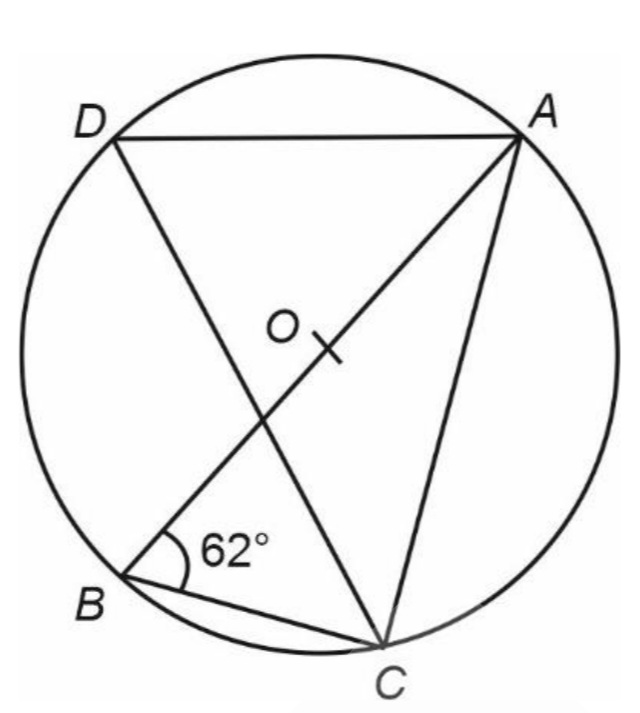
\includegraphics[width=\columnwidth]{figs/img5.jpg}
			\caption{}
			\label{figure}
		\end{figure}
\end{enumerate}  

%\section{2010}
%\subsection{12}
%\begin{enumerate}
	\item $ABCD$ is a cyclic quadrilateral. If $\angle BAD = (2x + 5)^{\circ}$ and $\angle BCD = (x + 10)^{\circ}$ then $x$ is equal to:
		\begin{figure}[h]
			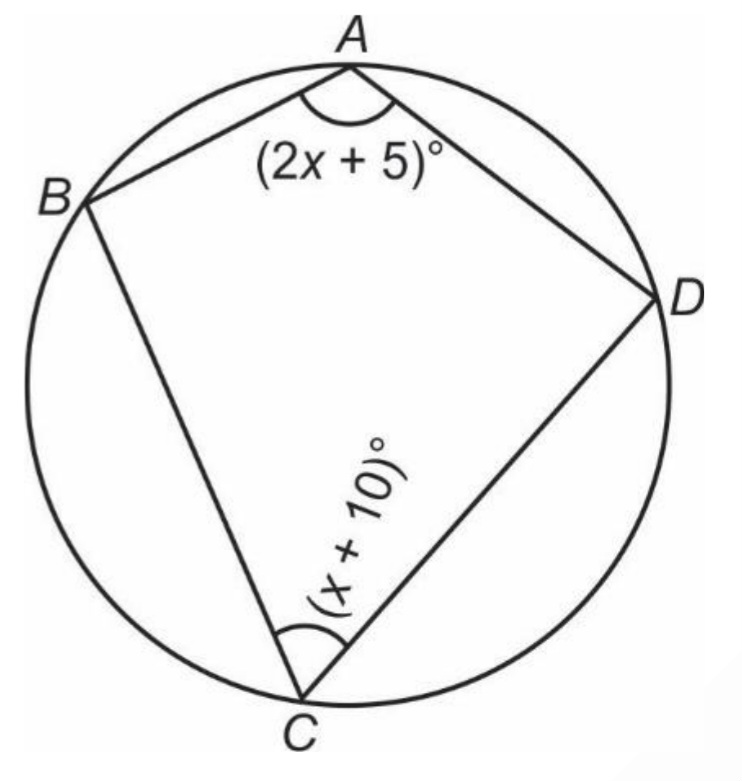
\includegraphics[width=\columnwidth]{figs/img2.jpg}
			\caption{}
			\label{figure}
		\end{figure}
		\begin{enumerate}
			\item $65^{\circ}$
			\item $45^{\circ}$
			\item $55^{\circ}$
			\item $5^{\circ}$
		\end{enumerate}
		\newpage
	\item In the given figure $O$ is the centre of the circle. $PQ$ and $PR$ are tangents and $\angle QPR = 70^{\circ}$. Calculate:
		{\begin{figure}[h]
			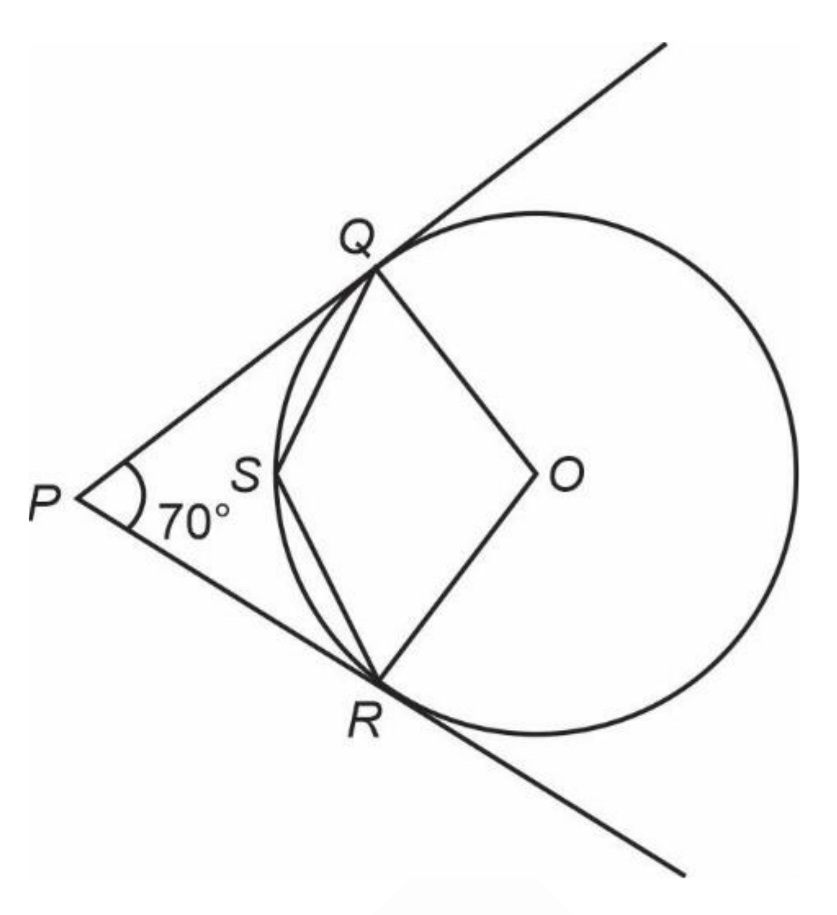
\includegraphics[width=\columnwidth]{figs/img3.jpg}
			\caption{}
			\label{figure}
		\end{figure}}
		\begin{enumerate}
			\item $\angle QOR$
			\item $\angle QSR$
		\end{enumerate}	
	\item Two chords $AB$ and $CD$ of a circle intersect extenally at $E$. if $EC = 2 cm$, $EA = 3 cm$ and $AB = 5 cm$, find the length of $CD$.
		\begin{figure}[h]
			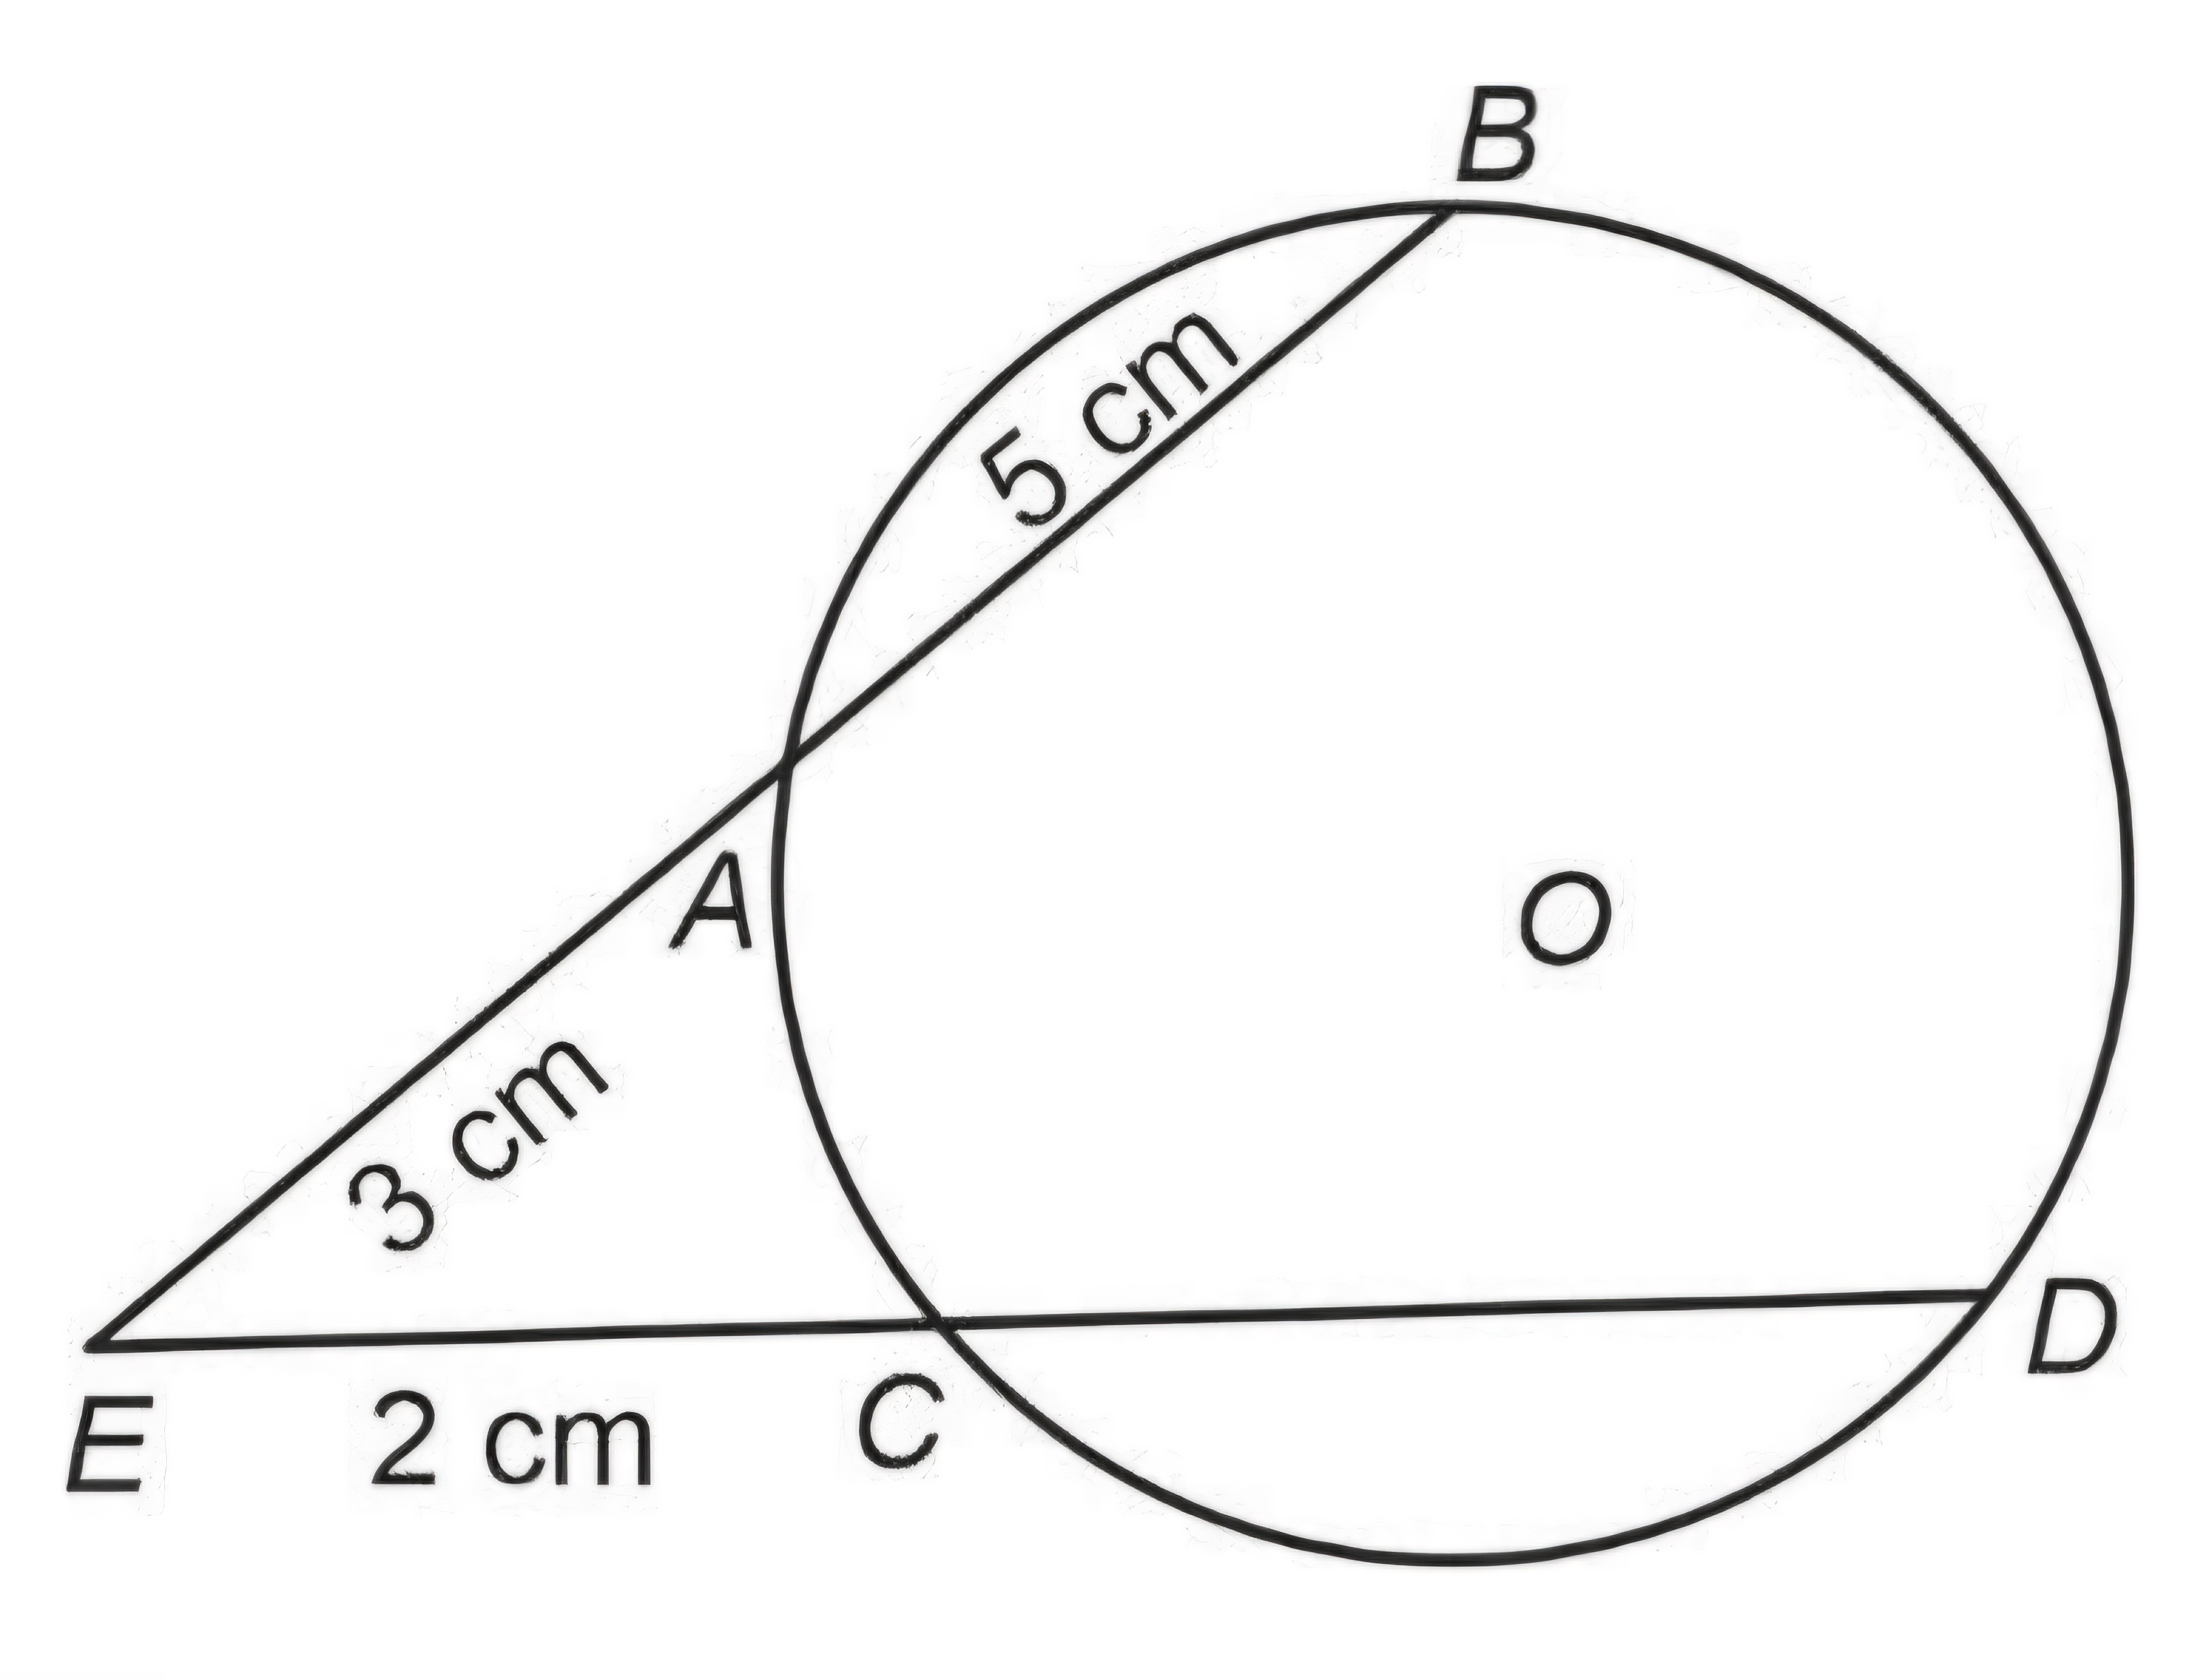
\includegraphics[width=\columnwidth]{figs/img4.jpg}
			\caption{}
			\label{figure}
		\end{figure}
		\newpage
	\item In the given figure $A,B,C$ and $D$ are points on the circle with centre $O$. Given $\angle ABS = 62^{\circ}$. Find:
		\begin{enumerate}
			\item $\angle ADC$
			\item $\angle CAB$
		\end{enumerate}
		\begin{figure}[h]
			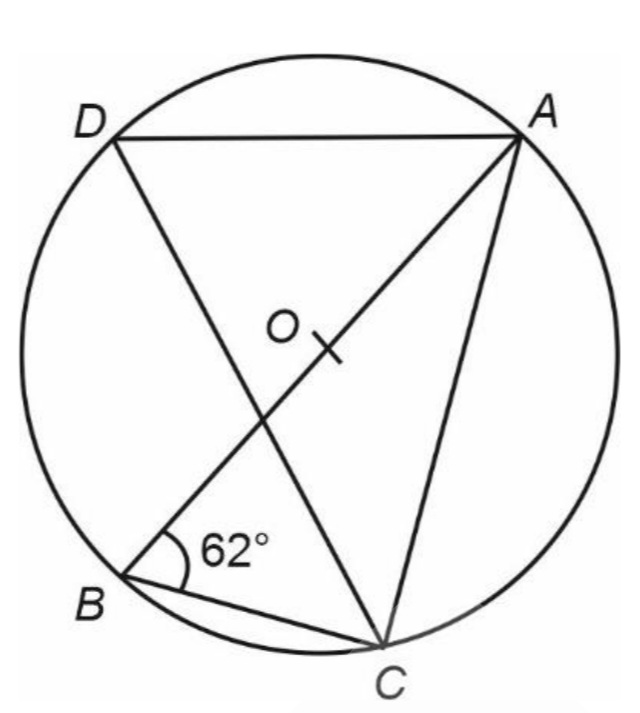
\includegraphics[width=\columnwidth]{figs/img5.jpg}
			\caption{}
			\label{figure}
		\end{figure}
\end{enumerate}  



\chapter{Intersection of Conics}

%\section{2010}
%\subsection{12}
%\input{2010/intersec.tex}





\chapter{Probability}
\section{2022}
\subsection{10}
 \begin{enumerate}
         \item The probability of getting a number divisible by $3$ in throwing a dice is:
		 \begin{enumerate}
		 \item $\frac{1}{6}$
		 \item $\frac{1}{3}$
		 \item $\frac{1}{2}$
		 \item $\frac{2}{3}$
		 \end{enumerate}
	 \item A bag contains $5$ white, $2$ red and $3$ black balls. A ball is drawn at random. What is the probability that the ball drawn is a red ball?
	 \item A letter of the word $"SECONDARY"$, is selected at random. What is the probability that the letter selected is not a vowel?
 \end{enumerate}


%\section{2010}
%\subsection{12}
%\input{2010/prob.tex}

\chapter{Construction}

%\section{2010}
%\subsection{12}
%\input{2010/construction.tex}


\chapter{Optimization}

%\section{2010}
%\subsection{12}
%\input{2010/opt.tex}


\chapter{Algebra}

%\section{2010}
%\subsection{12}
%\input{2010/algebra.tex}

\chapter{Geometry}
\section{2022}
\subsection{10}
 \begin{enumerate}
	 \item A lighthouse is $80 m$ high. The angle of elevation of its top from a point $80 m$ away from its foot along the same horizontal line is:
		 \begin{enumerate}
			 \item $60^{\circ}$
			 \item $45^{\circ}$
			 \item $30^{\circ}$
			 \item $90^{\circ}$
		 \end{enumerate}
	 \item Two lamp posts $AB$ and $CD$ each of height $100 m$ are on either side of the road. $P$ is a point on the road between the two lamp posts. The angle of elevation of the top of the lamp posts from te point $P$ are $60^{\circ}$ and $40^{\circ}$. Finf the distances $PB$ and $CD$.
 \end{enumerate}  

%\section{2023}
%\subsection{10}
%\input{2023/ASSIGNMENT_1.tex}

\chapter{Coordinate Geometry}
\section{2022}
\subsection{10}
\begin{enumerate}
	\item If two lines are perpendicular to one another then the relation between their slopes $m_{1}$ and $m_{2}$ is:
		\begin{enumerate}
			\item $m_{1} = m_{2}$
			\item $m_{1} = \frac{1}{m_{2}}$
			\item $m_{1} = -m_{2}$
			\item $m_{1} \times m_{2} = -1$
		\end{enumerate}
	\item The coordinates of the point $P(-3,5)$ on reflecting on the $x$-axis are:
		\begin{enumerate}
			\item $(3, 5)$
			\item $(-3, -5)$
			\item $(3, -5)$
			\item $(-3, 5)$
		\end{enumerate}
	\item $A(1, 4), B(4, 1)$ and $C(x, 4)$ are the vertices of $\bigtriangleup ABC$. If the centroid of the triangle is $G(4, 3)$ then $x$ is equal to:
		\begin{enumerate}
			\item $2$
			\item $1$
			\item $7$
			\item $4$
		\end{enumerate}
	\item Find $'a'$, if $A(2a + 2, 3$, $B(7,4)$ ad $C(2a +5, 2)$ are collinear.
	\item Find a point $P$ which divides internally the line segment joining the points $A(-3, 9)$ and $B(1, -3)$ in the ratio $1:3$.
	\item Use a graph paper for this question. Take $2 cm = 1$ unit along both the axes\\
		\begin{enumerate}
			\item Plot the points $A(0, 4), B(2, 2), C(5,2)$ and $D(4,0)$. $E(0, 0)$ is the origin.
			\item Reflect $B, C, D$ on the $y$-axis and name them as $B', C', D'$ respectively.
			\item Join the points $ABCDD'C'B'$ and $A$ in order and give a geometrical name to the closed figure.
		\end{enumerate}
	\item Find the equation of a line parallel to the line $2x + y - 7 = 0$ and passi    ng through the intersection of the lines $x + y- 4 =0$ and $2x - y =8$.
	\item Line $AB$ is perpendicular to $CD$. Coordinates of $B, C and D$ are respectively $(4, 0), (0, -1)$ and $(4,3)$.
		\begin{figure}[h]
			\centering
			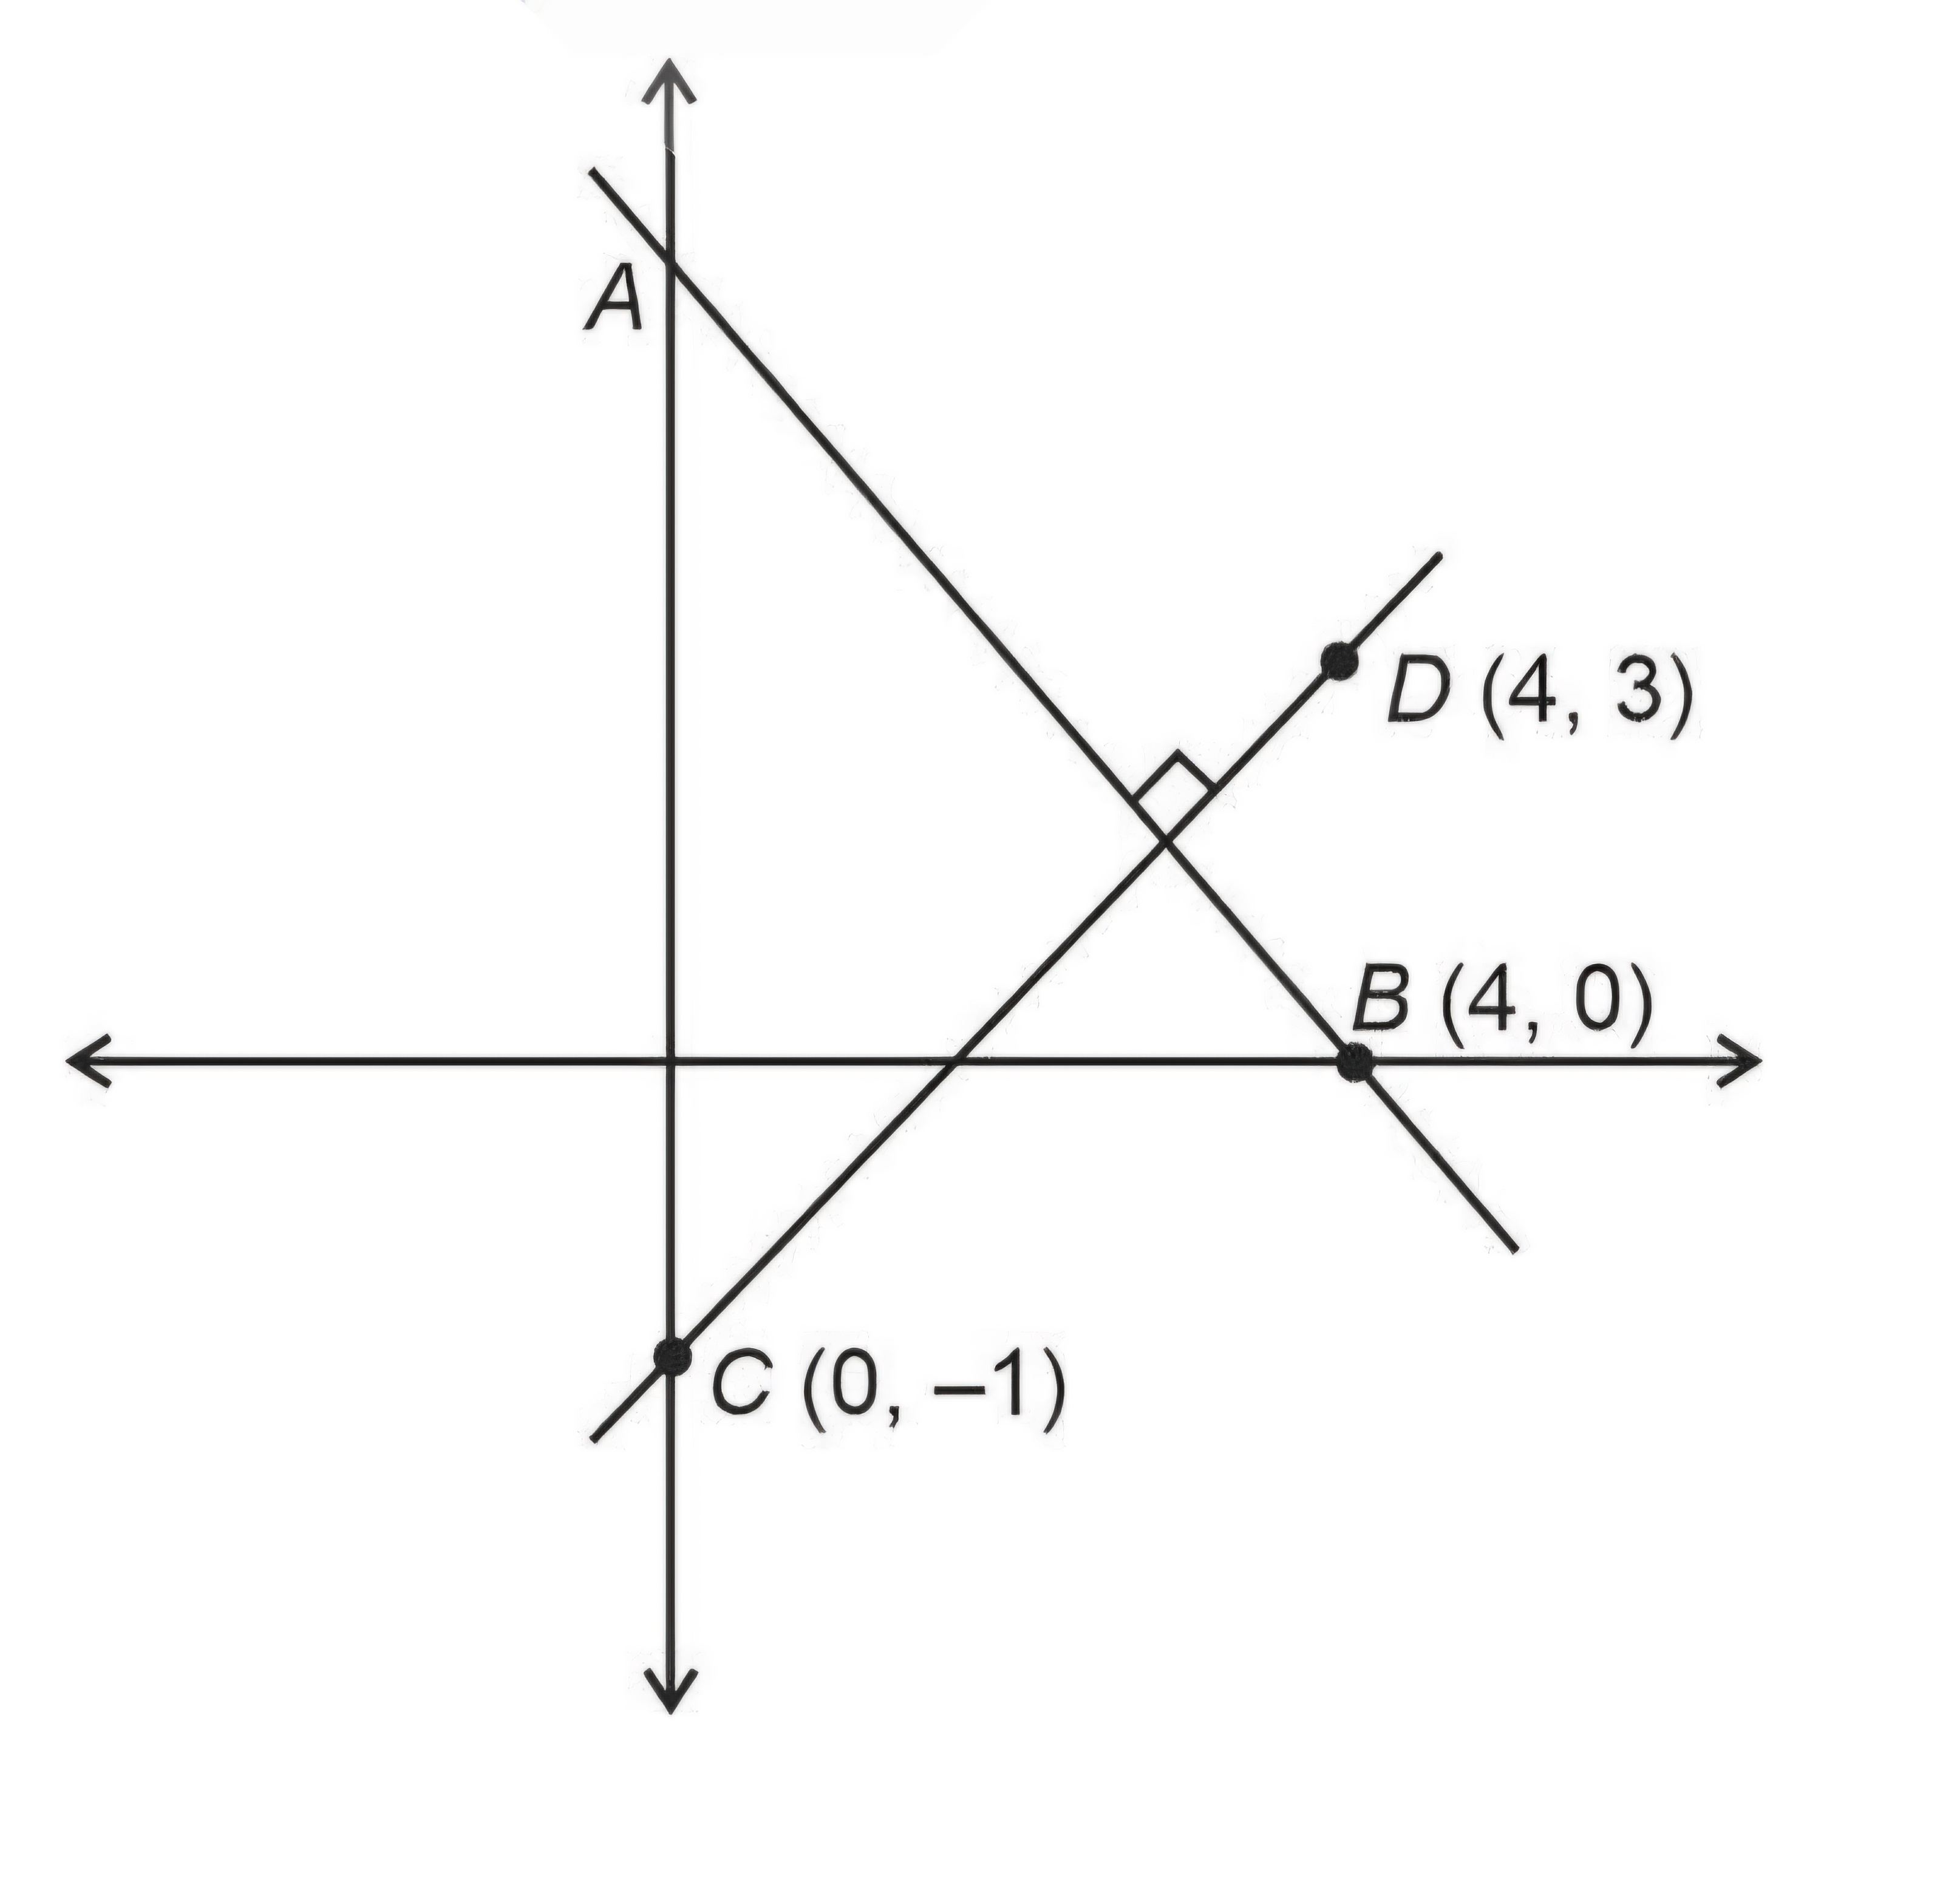
\includegraphics[width=\columnwidth]{figs/img6.jpg}
			\caption{}
			\label{figure}
		\end{figure}
		Find:
		\begin{enumerate}
			\item Slope of $CD$
			\item Equation of $AB$
		\end{enumerate}
\end{enumerate}


\chapter{3D-Geometry}
\section{2022}
\subsection{10}
 \begin{enumerate}
	 \item The volume of a conical tent is $462 m^{3}$ and the area of the base is $154 m^{2}$. The height of the cone is:
		 \begin{enumerate}
			 \item $15 m$
			 \item $12 m$
			 \item $9 m$
			 \item $24 m$
		 \end{enumerate}
	 \item The radius of a roller $100 cm$ long is $14 cm$. The curved surface area of the roller is: $(Take \pi = \frac{22}{7})$
		 \begin{enumerate}
			 \item $13200 cm^{2}$
			 \item $15400 cm^{2}$
			 \item $4400 cm^{2}$
			 \item $8800 cm^{2}$
		 \end{enumerate}
	 \item A solid cone of radius $5 cm$ and height $9 cm$ is melted and made into small cyliders of radius of $0.5 cm$ and height $1.5 cm$. Find the number of cylinders so formed.
	 \item A solid wooden cylinder is of radius $6 cm$ and height $16 cm$. Two cones ech of radius $2 cm$ and height $6 cm$ are drilled out of the cylinder. Find the volume of the remainiing solid.\\
		 \begin{figure}[h]
			 \centering
			 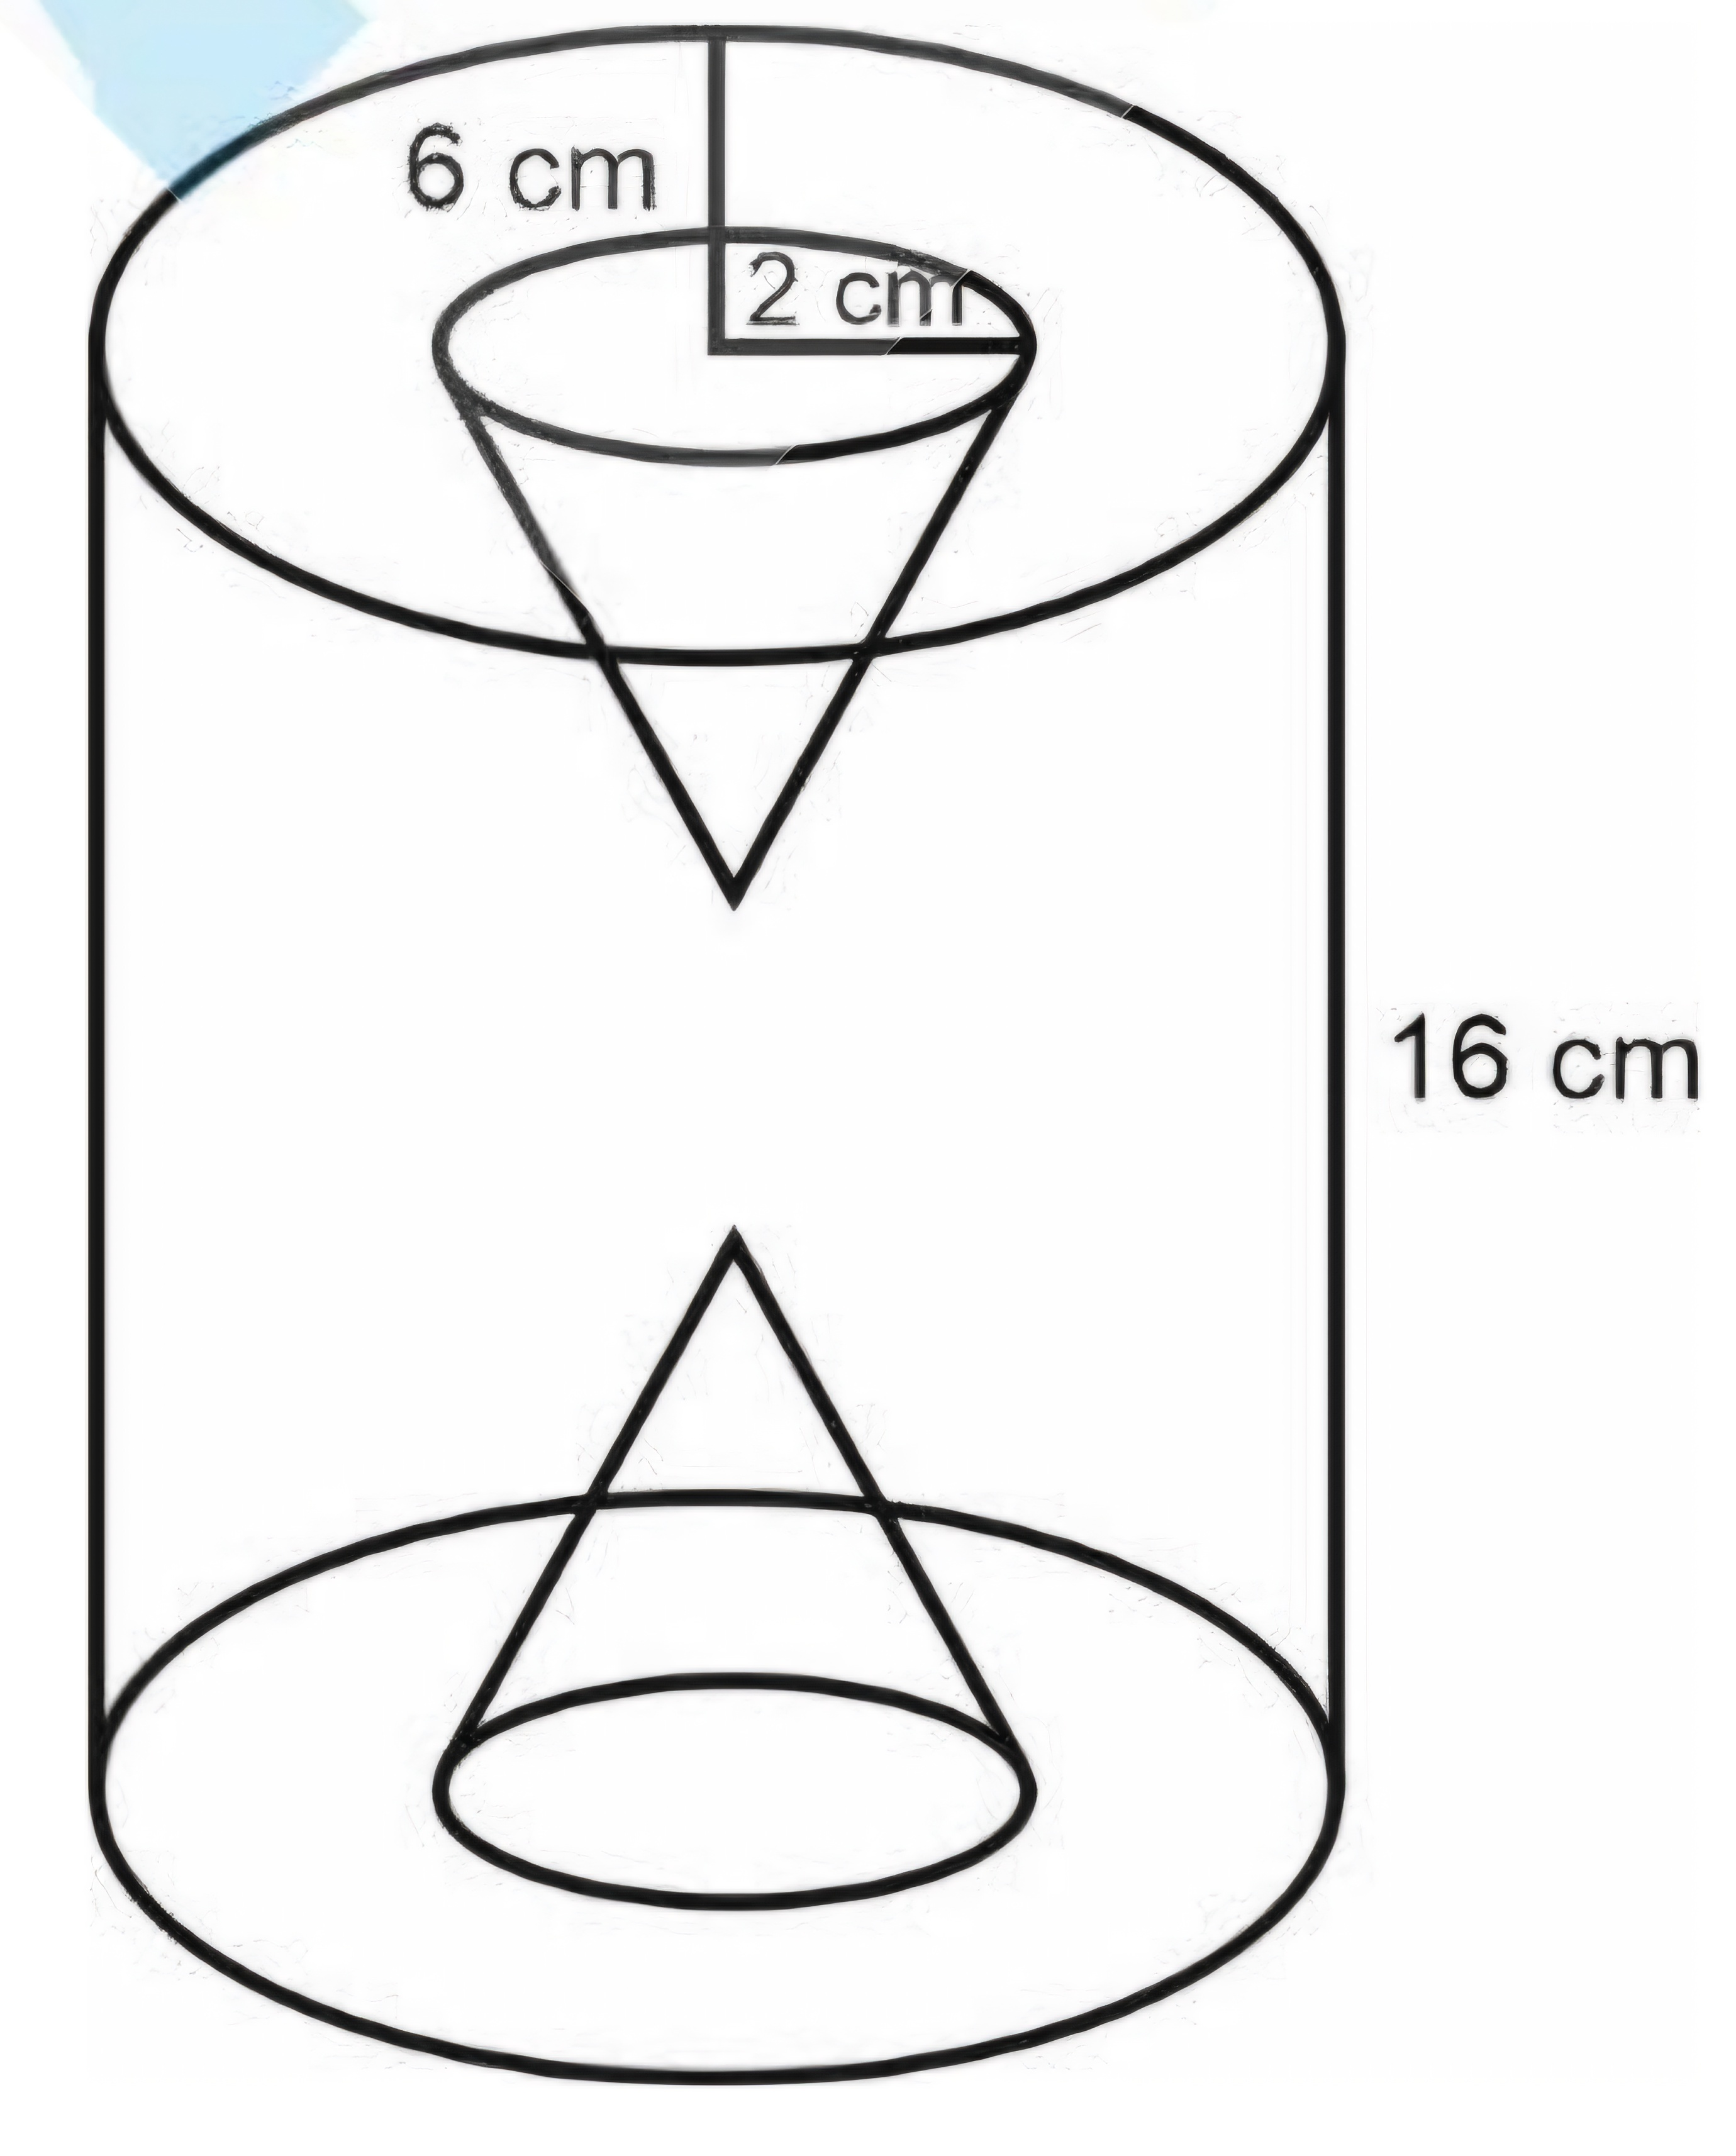
\includegraphics[width=\columnwidth]{figs/img1.jpg}
			 \caption{}
			 \label{Figure}
		 \end{figure}
 \end{enumerate}


\chapter{Discrete}
%\section{2010}
%\subsection{12}
%\input{2010/discrete.tex}

\chapter{Number Systems}
%\section{2010}
%\subsection{12}
%\input{2010/numbersys.tex}


\chapter{Differentiation}
%\section{2023}
%\subsection{12}
%\input{2023/differentiation.tex}






\chapter{Integration}
%\section{2010}
%\subsection{12}
%\input{2010/integrate.tex}


\chapter{Functions}
%\section{2023}
%\subsection{12}
%\input{2023/Functions.tex}




\chapter{Matrices}
%\section{2020}
%\subsection{10}
%\input{2020/mat10.tex}

\chapter{Data-Handling}
\section{2022}
\subsection{10}
\begin{enumerate}
	\item The median class for the given distribution is:\\
		\centering
		\begin{tabular}{|c|c|}
			\hline
			Class Interval & Frequency \\
			\hline
			0-10 & 2 \\
			10-20 & 4\\
			20-30 & 3\\
			30-40 & 5\\ 
			\hline
		\end{tabular}
		\begin{enumerate}
			\item $0-10$
			\item $10-20$
			\item $20-30$
			\item $30-40$
		\end{enumerate}
	\item The modal class of a given distribution always corresponds to the:
		\begin{enumerate}
			\item interval with highest frequency 
			\item interval with lowest frequency
			\item the first interval
			\item the last interval
		\end{enumerate}
	\item Calculate the mean of the following frequency distribution.\\
		\centering
		\begin{tabular}{|c|c|}
			\hline
			Class Interval & Frequency \\
			\hline
			5-15 & 2 \\
			15-25 & 6 \\
			25-35 & 4 \\
			35-45 & 8 \\
			45-55 & 4\\
			\hline
		\end{tabular}
	\item Marks obtained by 100 students in an examination are given below.
		\centering
		\begin{tabular}{|c|c|}
			\hline
			Marks & No. of students \\
			\hline
			0-10 & 5 \\
			10-20 & 15 \\
			20-30 & 20 \\
			30-40 & 28 \\
			40-50 & 20 \\
			50-60 & 12 \\
			\hline
		\end{tabular}
		\\Draw a histogram for the given data using a graph paper and find the mode. Take $2 cm = 10$ marks along one axis and $2 cm= 10$ students along the other axis.
	\item The mean of the following distribution is $50$. Find the unknown frequency.
		\centering
		\begin{tabular}{|c|c|}
			\hline
			Class Interval & Frequency \\
			\hline
			0-20 & 6 \\
			20-40 & f \\
			40-60 & 8 \\
			60-80 & 12 \\
			80-100 & 8 \\
			\hline
		\end{tabular}
	\item Marks obtained by $40$ students in an examination are given below.
		\centering
		\begin{tabular}{|c|c|}
			\hline
			Marks & No. of students \\
			\hline
			10-20 & 3 \\
			20-30 & 8 \\
			30-40 & 14 \\
			40-50 & 9 \\
			50-60 & 4 \\
			60-70 & 2 \\
			\hline
		\end{tabular}
		\\Using graph paper draw an ogive and estimate the median marks. Take $2 cm = 10$ marks along one axis and $ 2cm = 5$ students along the other axis.
\end{enumerate}


\chapter{Trignometry}
\section{2022}
\subsection{10}
 \begin{enumerate}
	 \item Prove that:\\
		 $\frac{1}{1 + \sin\theta}$ $+$ $\frac{1}{1 - \sin\theta}$ $=$ $2\sec^{2}\theta$
	 \item Prove that:\\
		 $\frac{(1 + \sin\theta)^{2} + (1 - \sin\theta)^{2}}{2\cos^{2}\theta}$ $=$ $\sec^{2}\theta + \tan^{2}\theta $
	 \item Prove that:\\
		 $1 + \frac{\tan^{2}\theta}{1 + \sec\theta} = \sec\theta$
 \end{enumerate}

%\section{2019}
%\subsection{10}
%\input{2019/trignj.tex}


%\include{ch02} 
\backmatter
\appendix
\iffalse
\chapter{Conic Lines}
\section{Pair of Straight Lines}
%
\input{quad/pair.tex}
\section{Intersection of Conics}
\input{quadlines/inter.tex}
\section{ Chords of a Conic}
\input{quadlines/chord.tex}
\section{ Tangent and Normal}
\input{quadlines/tangent.tex}
\fi
%\chapter{Proofs}
%   \section{}
%\input{apps/defs.tex}

%  \section{}
%\input{apps/parab.tex}
%  \section{}
%\input{apps/nonparab.tex}
%		\section{}
%\input{apps/params.tex}
\latexprintindex

\end{document}

 
\section{Examples}
\subsection{Loney}
\input{examples/loney.tex}
\subsection{Miscellaneous}
\input{examples/misc.tex}
%
%%\section*{Disclosure Statement}
%%The authors report there are no competing interests to declare.
%%
%%
%%
%%  
%%%All the results related to conics are summarized in 
%%%Table \ref{table:conics}.  
%%%\begin{table*}[!t]
%%%\centering
%%%\input{conics.tex}
%%%%\input{./figs/conics.tex}
%%%\caption{$\vec{x}^{\top}\vec{V}\vec{x}+2\vec{u}^{\top}\vec{x}+f = 0$  can be expressed in the above standard form for various conics. $\vec{c}$ represents the centre/vertex of the conic. $\vec{q}$ is/are the point(s) of contact for the tangent(s). }
%%%\label{table:conics}
%%%\end{table*}
%%%\begin{verbatim}
%%\bibliographystyle{tfs}
%%%\bibliography{interacttfssample}
%%\bibliography{school}
%%\end{verbatim}
%% included where the list of references is to appear, where \texttt{tfs.bst} is the name of the \textsc{Bib}\TeX\ bibliography style file for Taylor \& Francis' Reference Style S and \texttt{interacttfssample.bib} is the bibliographic database included with the \textsf{Interact}-TFS \LaTeX\ bundle (to be replaced with the name of your own .bib file). \LaTeX/\textsc{Bib}\TeX\ will extract from your .bib file only those references that are cited in your .tex file and list them in the References section.
%
%% Please include a copy of your .bib file and/or the final generated .bbl file among your source files if your .tex file does not contain a reference list in a \texttt{thebibliography} environment.
%

  % \section{Appendices}
  % \appendix

\appendices
